% =====================================================================
%  DL-Seminar handout — Agglomerative Multi-Teacher Knowledge Distillation
%  Compile:  pdflatex handout.tex   (or upload to Overleaf)
%  Needs: tikz, amsmath, booktabs, geometry, enumitem, titlesec, hyperref
% =====================================================================
\documentclass[10pt]{article}

\usepackage[a4paper,margin=1.6cm]{geometry}
\usepackage{amsmath,amssymb}
\usepackage{booktabs}

% --- colours (define BEFORE titlesec/hyperref use them) ---
\usepackage{xcolor}
\definecolor{tealblue}{RGB}{0,110,135}
\definecolor{teachercol}{RGB}{198,120,40}
\definecolor{studentcol}{RGB}{40,120,180}
\definecolor{lightgray}{RGB}{244,244,244}

\usepackage{tikz}
\usetikzlibrary{arrows.meta,positioning}

\usepackage{enumitem}
\setlist{nosep,leftmargin=1.2em}

\usepackage{titlesec}
\titlespacing*{\section}{0pt}{6pt}{2pt}
\titlespacing*{\subsection}{0pt}{4pt}{1pt}
\titleformat{\section}{\large\bfseries\color{tealblue}}{\thesection}{0.5em}{}
\titleformat{\subsection}{\normalsize\bfseries}{}{0em}{}

\usepackage[colorlinks=true,linkcolor=tealblue,urlcolor=tealblue,citecolor=tealblue]{hyperref}

\setlength{\parindent}{0pt}
\setlength{\parskip}{2pt}
\pagestyle{empty}

% info box for explaining *why* we do something (not for stating extra facts)
\newcommand{\whybox}[1]{%
  \par\smallskip\noindent
  \fcolorbox{tealblue}{lightgray}{%
    \begin{minipage}{\dimexpr\linewidth-2\fboxsep-2\fboxrule\relax}
    #1
    \end{minipage}}%
  \par\smallskip}

\begin{document}

% =====================  HEADER  =====================
\begin{center}
{\LARGE\bfseries From Many Experts to One}\\[2pt]
{\large Agglomerative Multi-Teacher Knowledge Distillation}\\[3pt]
{\small DL-Seminar handout \;\textbar\; case study: \texttt{patho-distill} — distilling pathology foundation models}
\end{center}
\vspace{-3pt}\hrule\vspace{4pt}

% =====================  BACKGROUND  =====================
\section{Background}

Large models pre-trained with self-supervision on broad image corpora—commonly termed
\emph{foundation models}—have become a widely used transfer-learning substrate across several
areas of computer vision~\cite{bommasani}. In computational pathology their appeal is concrete:
expert annotations are scarce and costly to obtain, gigapixel whole-slide images make training an
encoder from scratch computationally prohibitive, and a single reusable encoder can serve many
downstream tasks~\cite{moor,uni}. Several such encoders are now available. The three we study
here—UNI2-h~\cite{uni}, Virchow2~\cite{virchow2}, and H-optimus-1~\cite{hoptimus}—are Vision
Transformers (ViTs) with $0.6$--$1.1$\,B parameters, and they are a deliberate selection from a
larger and growing pool. Because these encoders differ in their pre-training data and training
recipes, their representations are not interchangeable: measured performance varies systematically
across tissue types and downstream tasks~\cite[Fig.~1]{pathryoshka}.

% =====================  OBJECTIVE  =====================
\section{Objective}

For this seminar series we assess the feasibility of obtaining a single, compact pathology
encoder that inherits the complementary strengths of several specialised teachers, replacing
several large forward passes with one. We approach this with multi-teacher \emph{knowledge
distillation}: training one small model to reproduce the representations of several large
ones~\cite{hinton,radio}.

% =====================  DATA  =====================
\section{Data}

The distillation targets are the teachers' own embeddings rather than human labels, so the
procedure requires only raw image tiles~\cite{radio}; in pathology, unlabelled tissue tiles are
available at very large scale, as the teachers' own pre-training corpora illustrate
(${>}200$\,M tiles for UNI2-h)~\cite{uni}. We stream ${\sim}248$\,GB of unlabelled H\&E tiles
(51 WebDataset shards, $256\times256$\,px, cropped to $224\times224$) directly from object storage,
holding out one shard for validation.

% =====================  METHODOLOGY  =====================
\section{Methodology}

\emph{Knowledge distillation}, as proposed by Hinton et al.~\cite{hinton}, trains a small
\emph{student} to imitate a large frozen \emph{teacher} by matching the teacher's output
logits (soft labels). We instead use \emph{feature distillation}: the student is trained to
reproduce the teacher's internal \emph{embedding}. We combine three teachers into one student
following AM-RADIO~\cite{radio}, an agglomerative approach that merges several teachers into a
single student encoder. Three design considerations follow; they are the transferable ideas.

\begin{enumerate}[label=\textbf{\arabic*.}]
\item \textbf{Teachers produce embeddings of different dimensionality.} UNI2-h and H-optimus-1
emit 1536-d vectors, Virchow2 1280-d, while the student is 768-d. The student therefore carries
\textbf{one small projection head (MLP) per teacher} that maps its 768-d features to that teacher's
dimension. The shared backbone learns a single union representation; each head reads off a
teacher-specific view of it.

\item \textbf{Global and local structure are matched separately.} A ViT emits a \texttt{CLS}
token, which provides a global summary of the analysed image, alongside one token per image patch
(here $16\times16=256$), which carry spatial feature relevance. We distil both: patch $i$ of the
student is matched to patch $i$ of each teacher (all use patch-size 14 at 224\,px, giving an
identical $16\times16$ grid).

\item \textbf{Teachers occupy different output distributions.} Raw embeddings differ markedly in
per-channel magnitude across teachers. This is remedied by \textbf{standardising} each teacher's
output (zero-mean, unit-variance per channel) before comparison, so that no single teacher
dominates the loss~\cite{radio}.
\end{enumerate}

% ---- architecture diagram ----
\begin{center}
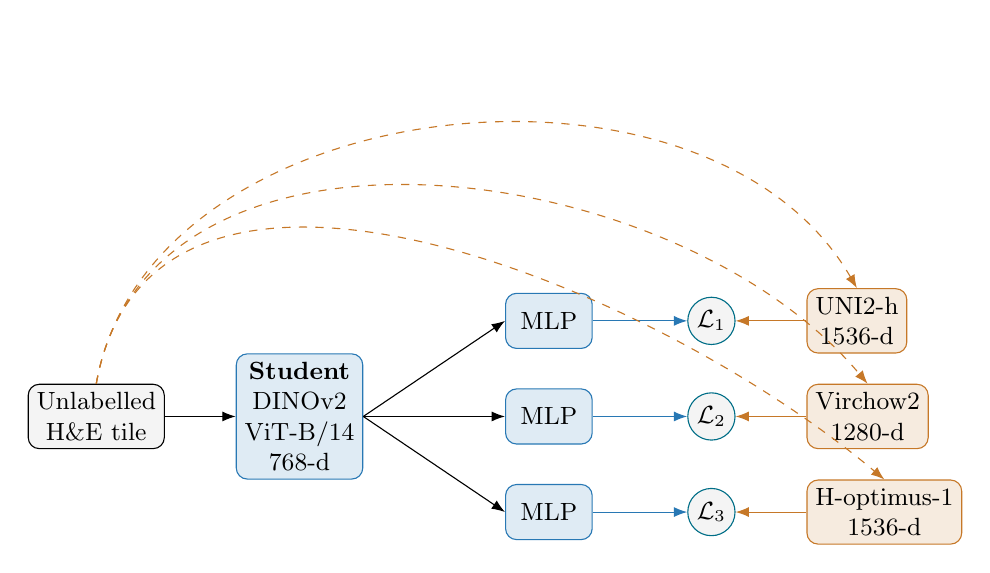
\begin{tikzpicture}[font=\small, >=Latex,
  box/.style={rounded corners,draw,minimum height=7mm,inner sep=3pt,align=center},
  tea/.style={box,fill=teachercol!15,draw=teachercol},
  stu/.style={box,fill=studentcol!15,draw=studentcol},
  mlp/.style={box,fill=studentcol!15,draw=studentcol,minimum width=11mm},
  loss/.style={circle,draw=tealblue,fill=lightgray,inner sep=1pt,minimum size=6mm}]

  \node[box,fill=lightgray] (img) {Unlabelled\\H\&E tile};
  \node[stu,right=9mm of img] (stud) {\textbf{Student}\\DINOv2\\ViT-B/14\\768-d};

  % stack of 3 per-teacher MLP heads (drawn as offset copies to read as a stack)
  \node[mlp,right=18mm of stud] (h2) {MLP};
  \node[mlp,above=5mm of h2]    (h1) {MLP};
  \node[mlp,below=5mm of h2]    (h3) {MLP};

  % loss nodes
  \node[loss,right=12mm of h1] (l1) {$\mathcal{L}_1$};
  \node[loss,right=12mm of h2] (l2) {$\mathcal{L}_2$};
  \node[loss,right=12mm of h3] (l3) {$\mathcal{L}_3$};

  % frozen teachers
  \node[tea,right=9mm of l1] (t1) {UNI2-h\\1536-d};
  \node[tea,right=9mm of l2] (t2) {Virchow2\\1280-d};
  \node[tea,right=9mm of l3] (t3) {H-optimus-1\\1536-d};

  \draw[->] (img) -- (stud);
  \draw[->] (stud.east) -- (h1.west);
  \draw[->] (stud.east) -- (h2.west);
  \draw[->] (stud.east) -- (h3.west);
  \draw[->,studentcol] (h1) -- (l1);
  \draw[->,studentcol] (h2) -- (l2);
  \draw[->,studentcol] (h3) -- (l3);
  \draw[->,teachercol] (t1) -- (l1);
  \draw[->,teachercol] (t2) -- (l2);
  \draw[->,teachercol] (t3) -- (l3);
  % same tile feeds the frozen teachers (arc over the top)
  \draw[->,teachercol,dashed] (img.north) to[out=80,in=120] (t1.north);
  \draw[->,teachercol,dashed] (img.north) to[out=80,in=130] (t2.north);
  \draw[->,teachercol,dashed] (img.north) to[out=80,in=140] (t3.north);
\end{tikzpicture}\\[3pt]
{\footnotesize\itshape Figure 1. The same frozen tile is encoded by the student and by each
frozen teacher. One MLP head per teacher (three in total) projects the student's 768-d
\texttt{CLS} and patch tokens to that teacher's dimension; each loss $\mathcal{L}_t$ is formed
between the projected student tokens and the teacher's standardised tokens. Only the student and
its three heads are trained.}
\end{center}

\subsection{The loss}

For each teacher $t$ we compare the student's projected tokens $s$ to the teacher's standardised
tokens $\hat y_t$, over both the \texttt{CLS} summary and the patch tokens:
\[
\mathcal{L}_t=\underbrace{\big(1-\cos(s^{\text{cls}},\hat y_t^{\text{cls}})\big)}_{\text{summary: direction}}
+\underbrace{\big(1-\cos(s^{\text{pat}},\hat y_t^{\text{pat}})\big)}_{\text{patches: direction}}
+\underbrace{\text{smooth-}L_1(s^{\text{pat}},\hat y_t^{\text{pat}})}_{\text{patches: magnitude}},
\qquad
\mathcal{L}=\!\!\sum_{t\in\text{teachers}}\!\!\mathcal{L}_t .
\]
The cosine term constrains the orientation of the student's token vectors to match the teacher's;
the smooth-$L_1$ term additionally constrains their magnitude. Optimising both reproduces the
teacher's representation geometry rather than only its directional structure.

\subsection{Training setup}

The student is a DINOv2 ViT-B/14 backbone with register tokens (86.6\,M parameters)~\cite{dinov2}.
Only the student backbone and its three projection heads are optimised; all teachers stay frozen.
We optimise with AdamW~\cite{adamw} at a peak learning rate of $10^{-4}$ and weight decay $0.05$,
batch size 64, with gradients clipped to norm 1.0. The learning rate follows a linear warmup over
the first 2\,000 steps to its peak, then a cosine decay toward zero over the remaining
steps~\cite{sgdr}. The summary and patch losses are weighted equally ($w=1$ each) and summed over
the three teachers. Training uses fp16 mixed precision~\cite{amp}: on the Volta-generation V100,
bf16 is emulated and substantially slower, so fp16 is the appropriate setting. The run targets
100k steps on a single V100.

% =====================  RESULTS  =====================
\section{Results}

We assess representation quality by \emph{linear probing} with Kaiko \texttt{eva}~\cite{eva}: the
student is frozen, its embeddings are extracted, and a linear classifier is trained on a labelled
task — here BACH (4-class breast histology)~\cite{bach}. The same protocol is applied to each
teacher for comparison. We report accuracy as mean $\pm$ standard deviation over five probe runs,
with the best result in bold.

\whybox{\textbf{Results in progress.} The final BACH readings for the student's last checkpoint and
for all three teachers are still being computed under the identical \texttt{eva} protocol; the table
below will be completed once they are available. We defer interpretation until then.}

\begin{center}
\begin{tabular}{lcc}
\toprule
Model & Params & BACH accuracy (\%) \\
\midrule
UNI2-h~\cite{uni}        & 681\,M & TBD \\
Virchow2~\cite{virchow2} & 632\,M & TBD \\
H-optimus-1~\cite{hoptimus} & 1.1\,B & TBD \\
\midrule
Student (ours)           & 86.6\,M & TBD \\
\bottomrule
\end{tabular}
\end{center}

{\footnotesize\itshape BACH is a small 4-class task that probes only the \texttt{CLS} embedding and
is excluded from the public \texttt{eva} leaderboard; the teachers are therefore benchmarked under
the identical protocol rather than cited from the leaderboard. Dense and slide-level (MIL) tasks
are not yet evaluated. A companion notebook (\texttt{demo.ipynb}) gives a self-contained, CPU-only
reproduction of the loss and linear-probe pipeline.}

% =====================  REFERENCES  =====================
\vspace{2pt}\hrule\vspace{2pt}
{\footnotesize
\begin{thebibliography}{9}
\setlength{\itemsep}{0pt}
\bibitem{bommasani} Bommasani \emph{et al.}, On the Opportunities and Risks of Foundation Models. arXiv:2108.07258, 2021.
\bibitem{moor} Moor \emph{et al.}, Foundation models for generalist medical artificial intelligence. \emph{Nature} 616, 2023.
\bibitem{uni} Chen \emph{et al.}, Towards a general-purpose foundation model for computational pathology (UNI). \emph{Nat. Med.} 30, 2024.
\bibitem{virchow2} Zimmermann \emph{et al.}, Virchow2: Scaling Self-Supervised Mixed Magnification Models in Pathology. arXiv:2408.00738, 2024.
\bibitem{hoptimus} Bioptimus, H-optimus-1: a 1.1\,B-parameter ViT-g/14 pathology foundation model, 2025. \texttt{huggingface.co/bioptimus/H-optimus-1}.
\bibitem{radio} Ranzinger \emph{et al.}, AM-RADIO: Agglomerative Vision Foundation Models. CVPR 2024.
\bibitem{hinton} Hinton, Vinyals, Dean. Distilling the Knowledge in a Neural Network. NeurIPS Deep Learning Workshop 2015.
\bibitem{dinov2} Oquab \emph{et al.}, DINOv2: Learning Robust Visual Features without Supervision. TMLR 2024.
\bibitem{adamw} Loshchilov, Hutter. Decoupled Weight Decay Regularization (AdamW). ICLR 2019.
\bibitem{sgdr} Loshchilov, Hutter. SGDR: Stochastic Gradient Descent with Warm Restarts. ICLR 2017.
\bibitem{amp} Micikevicius \emph{et al.}, Mixed Precision Training. ICLR 2018.
\bibitem{eva} kaiko.ai, \texttt{eva} — an evaluation framework for pathology foundation models.
\bibitem{bach} Aresta \emph{et al.}, BACH: Grand Challenge on Breast Cancer Histology Images. \emph{Medical Image Analysis} 56, 2019.
\bibitem{pathryoshka} Grashei \emph{et al.}, Pathryoshka: Compressing Pathology Foundation Models via Multi-Teacher Knowledge Distillation with Nested Embeddings. arXiv:2511.23204, 2025.
\end{thebibliography}}

\end{document}
